\section{Activity Forecasting}

\logo
{
	\begin{tikzpicture}
		\hspace{0.09cm}
		\node at (-1,0) [draw=white,ultra thick,inner sep=0pt]
		{
			
\includegraphics[height=1cm]{ThemeFigs/Sapienza}
		};
		\node at (0,0) [draw=white,ultra thick,inner sep=0pt]
		{
			
\includegraphics[height=1cm]{ThemeFigs/Edinburgh}
		};
	\end{tikzpicture}
	\vspace{199.1pt}
}

\begin{frame}
	\frametitle{Predicting Future Agent Motions}
	
	\vspace{0.2cm}
	
	\begin{block}{Idea}
		Performing activity forecasting resolving an \textbf{Inverse Reinforcement Learning} problem
		\textbf{without} needing a labelled environment, by combining:
		\vspace{0.05cm}
		\begin{itemize}
			\item Object trajectories provided by \emph{PTracking}
			\item Representation of the environment following the \emph{grid world} schema defined by
				  Russell et al. \cite{Ng00}
		\end{itemize}
	\end{block}
	
	\vspace{-0.1cm}
	
	\begin{center}
		\begin{tikzpicture}
			\node at (0,0) [draw=white,ultra thick,inner sep=0pt]
			{
				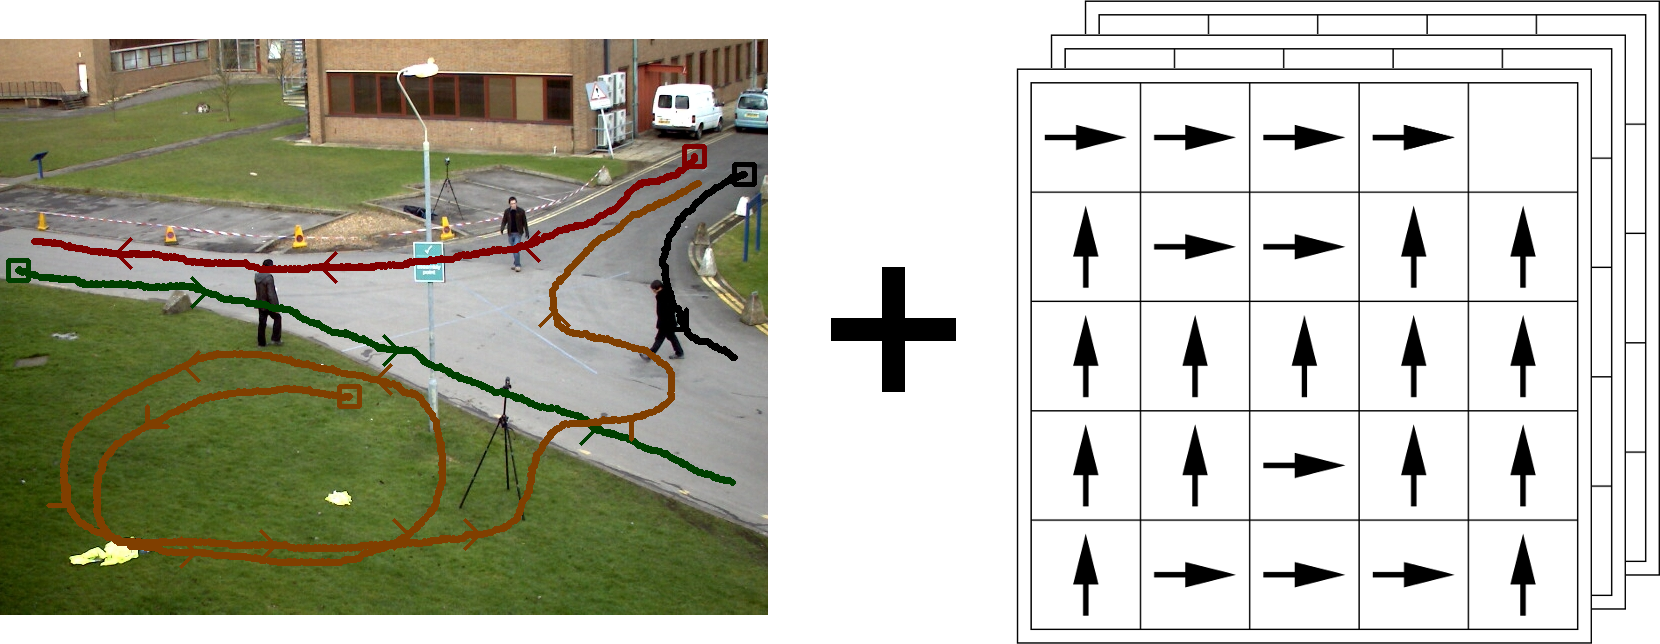
\includegraphics[height=3.2cm]{Figures/IRL}
			};
		\end{tikzpicture}
	\end{center}
	
	\vspace{-0.34cm}
	
	\tiny
	
	\cite{Ng00} S. Russell \emph{et al.},  ``Algorithms for inverse reinforcement learning'', ICML,
	2000
\end{frame}

\begin{frame}
	\frametitle{Predicting Future Agent Motions}
	\framesubtitle{Approach}
	
	\vspace{-0.1cm}
	
	\begin{columns}[T]
		\column{.4\textwidth}
		
		\vspace{-0.2cm}
		
		\begin{equation*}
			\hspace{0.3cm}
			\scriptsize
			\begin{array}{ll}
				\min \sum\nolimits_{i=1}^N -x_i + \lambda (r_i^+ - r_i^-)
				\vspace{-0.35cm} \\ \\
				s.t. \\ \;\;\;\;
				\left \{
					\begin{array}{ll}
						x_i \leq (\mathbf{P}_{a_*} - \mathbf{P}_a)(\mathbf{I} - \gamma
						\mathbf{P}_{a_*})^{-1} \mathbf{R} \\
						\vspace{-0.25cm} \\
						\;\;\;\;\;\;\;\;\;\;\;\;\;\;\;\;\;\;\;\;\;
						\;\;\; \forall \, a \in \mathbf{A}, \; i \in \{ 1, \ldots, N \}
						\vspace{-0.25cm}\\ \\
						x_i \geq 0 \;\;\;\;\;\;\,\,\,\,\;\;\;\,\,\,\,\,\;\,\,\,\,\,\,\,\;\;\;\;\;
						\;\,\,\,\,\, i \in \{ 1, \ldots, N \}
						\vspace{-0.25cm} \\ \\
						r_i = r_i^+ + r_i^- \;\,\,\,\,\,\;\,\,\,\,\,\,\,\;\;\;\;\;
						\;\,\,\,\,\, i \in \{ 1, \ldots, N \}
						\vspace{-0.25cm}
						\\ \\
						| \mathbf{R}_i | \leq R_{max} \;\;\;\;\;\;\;\;\;\;\;\,\,\,\,\;\;\
						\,\,\,\,\,\, i \in \{ 1, \ldots, N \}
					\end{array}
				\right.
				\vspace{0.2cm}
			\end{array}
		\end{equation*}
		
		\tiny
		
		\vspace{-0.8cm}
		
		\begin{tabbing}
			\hspace{0.2cm}
			Adapted formalisation of [Ng \& Russel, 2000]
		\end{tabbing}
		
		\vspace{-1cm}
		
		\column{.15\textwidth}
		
		\centering
		\vspace{1.3cm}
		
		\begin{tabbing}
			\hspace{1.5cm}
			\Huge
			\textcolor{red}{\textbf{+}}
		\end{tabbing}
		
		\column{.45\textwidth}
		\centering
		
		\vspace{0.4cm}
		
		\begin{tikzpicture}
			\node at (0,0) [draw=black,ultra thick,inner sep=0pt]
			{
				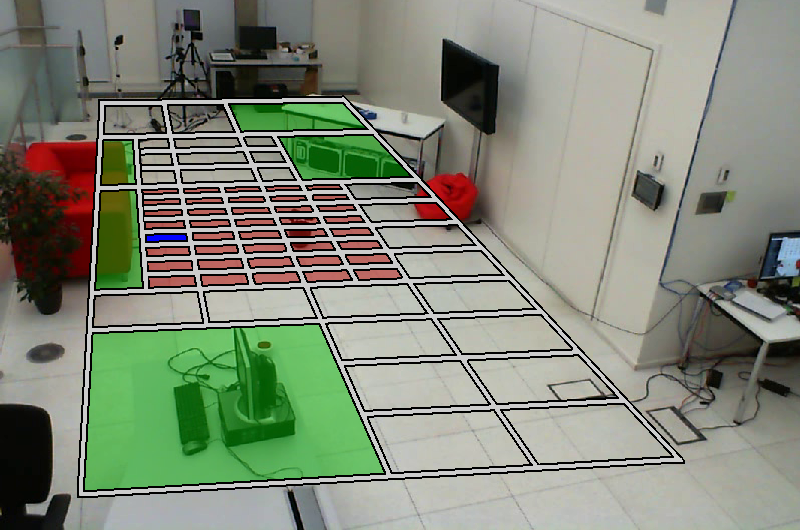
\includegraphics[width=4.8cm]{Figures/RecursiveNonUniformGrids}
			};
		\end{tikzpicture}
	\end{columns}
	
	\vspace{0.2cm}
	
	\begin{columns}[T]
		\column{.35\textwidth}
		
		\begin{tikzpicture}
			\hspace{0.2cm}
			\centering
			\node at (0,0) [draw=white,ultra thick,inner sep=0pt]
			{
				\includegraphics[height=3.2cm]{Figures/IRL-Model}
			};
		\end{tikzpicture}
		
		\column{.2\textwidth}
		
		\centering
		\vspace{1.1cm}
		
		\begin{tabbing}
			\hspace{1.975cm}
			\Huge
			\textcolor{red}{\textbf{$ \Rightarrow $}}
		\end{tabbing}
		
		\column{.45\textwidth}
		\centering
		
		\begin{tikzpicture}
			\node at (0,0) [draw=black,ultra thick,inner sep=0pt]
			{
				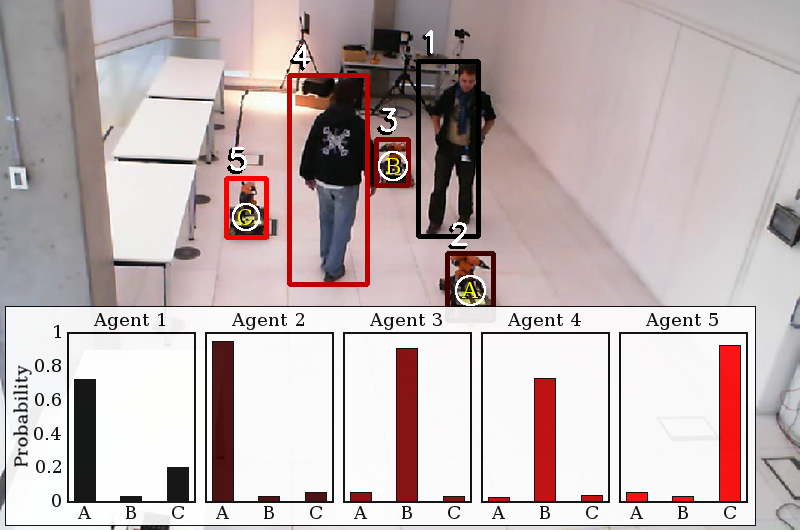
\includegraphics[width=4.8cm]{Figures/Motivation}
			};
		\end{tikzpicture}
	\end{columns}
	
	\begin{columns}[T]
		\column{\textwidth}
		
		\centering
		\vspace{-3.1cm}
		\hspace{-1cm}
		\Huge
		\begin{rotate}{-45}
			
			\textcolor{blue}{\textbf{$ \Downarrow $}}
		\end{rotate}	
	\end{columns}
\end{frame}

\begin{frame}
	\frametitle{Predicting Future Agent Motions}
	\framesubtitle{Policy Generation}
	
	\vspace{0.4cm}
	
	\begin{center}
		\begin{tikzpicture}
			\node at (-4.3,-1) [draw=black,ultra thick,inner sep=0pt]
			{
				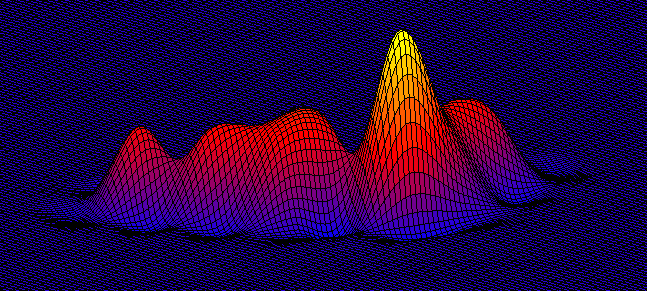
\includegraphics[width=0.5\linewidth]{Figures/Reward-3}
			};
			\node at (1,1) [draw=black,ultra thick,inner sep=0pt]
			{
				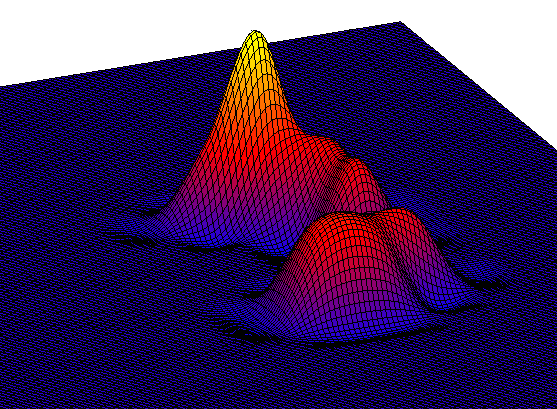
\includegraphics[width=0.45\linewidth]{Figures/Reward-2}
			};
			\node at (-4,1.7) [draw=black,ultra thick,inner sep=0pt]
			{
				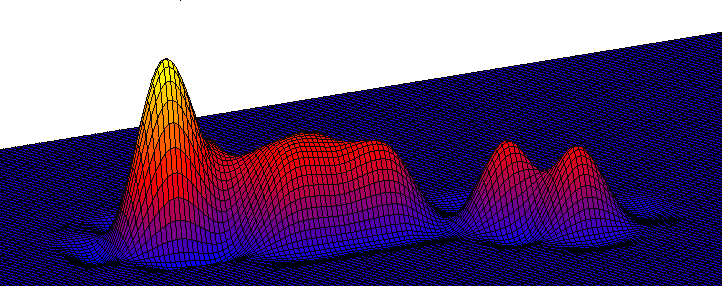
\includegraphics[width=0.5\linewidth]{Figures/Reward-1}
			};
		\end{tikzpicture}
	\end{center}
	
	\vspace{-0.1cm}
	
	\begin{center}
		Goals can be \emph{statically} chosen or \emph{generated} by analysing tracking data
	\end{center}
\end{frame}

\begin{frame}
	\frametitle{Predicting Future Agent Motions}
	\framesubtitle{Policy Comparison}
	
	\Large
	
	\vspace{0.3cm}
	
	Best fitting policy by \textbf{comparing} the target trajectory against trajectories drawn from
	potential optimal policies.
	
	\vspace{-0.3cm}
	
	\begin{center}
		\begin{tikzpicture}
			\node at (0,0) [draw=white,ultra thick,inner sep=0pt]
			{
				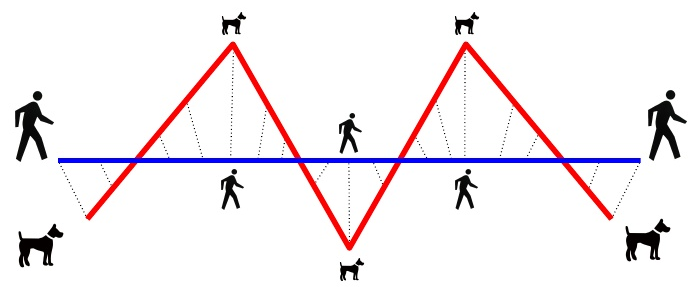
\includegraphics[width=0.72\linewidth]{Figures/Frechet}
			};
		\end{tikzpicture}
	\end{center}
	
	\vspace{-0.5cm}
	
	The \textbf{Fr\'echet distance} between curves is the minimum leash length that permits the walk.\\
\end{frame}

\begin{frame}
	\frametitle{Predicting Future Agent Motions}
	\framesubtitle{Goal Prediction}
	
	\Large
	
	\vspace{0.25cm}
	
	We \textbf{predict in real-time} the goal toward which each moving object is likely to be headed,
	by executing the policy that best matches its movement pattern.
	
	\vspace{-0.1cm}
	
	\begin{center}
		\begin{tikzpicture}
			\node at (0,0) [draw=black,ultra thick,inner sep=0pt]
			{
				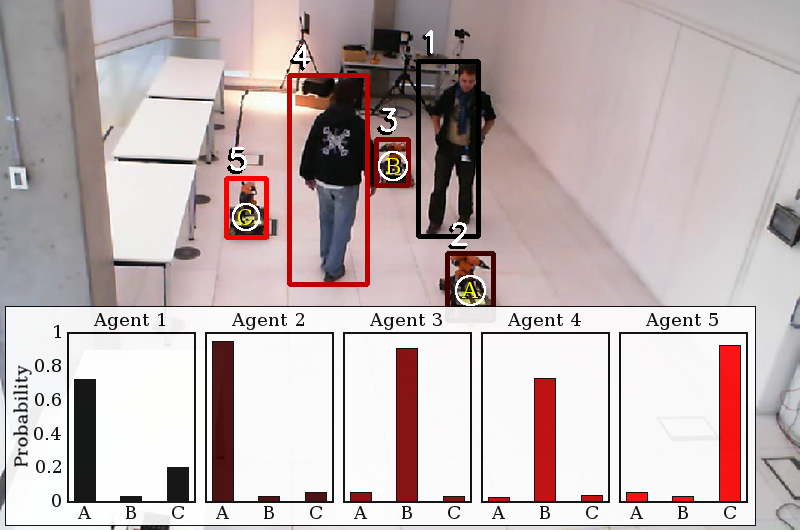
\includegraphics[width=0.59\linewidth]{Figures/Motivation}
			};
		\end{tikzpicture}
	\end{center}
\end{frame}
